\section{Auswertung}
\label{sec:Auswertung}
\subsection{Bestimmung der Brennweite über Gegenstands- und Bildweite.}
Zur Bestimmung der Brennweiten wird die Gleichung \eqref{eqn:LG} verwendent.
Die so erhaltenen Brennweiten werden gemittel. Daraus ergibt, dass die bestimmte
mittlere Brennweite $ \bar{f_{L}}$ für die Linse mit einer Brennweite von \SI{100}{\milli\meter}
\begin{equation*}
  \bar{f_{L}} = \SI{0.0983(4)}{\meter}
\end{equation*}
beträgt. Für die mittlere Brennweite der Wasserlinse $ \bar{f_{W}}$ ergibt
sich
\begin{equation*}
  \bar{f_{W}} = \SI{0.076(2)}{\meter} \; .
\end{equation*}
Die Darstellungen in Abbildung \ref{fig:gb} zeigen beide bei den entsprechen
den Werten für die jeweiligen Brennweiten einen ungefähren Häufungspunkt.
Der Abbildungsmaßstab wurde mit der Gleichung \eqref{eqn:AG} einmal mit
den Gegenstands- und Bildweiten und einmal mit den Gegenstands- und Bildgrößen
berechnet. Die so erhaltenen Abbildungsmaßstäbe wurden gemittel.
Die Gegenstandsgröße $G$ beträgt \SI{3}{\centi\meter}.
Dann ergbit sich für den mittleren Abbildungsmaßstab bestimmt über die
Gegenstands- und Bildweiten
\begin{equation*}
  \bar{V_{gb}} = \SI{1.5(6)}{}
\end{equation*}
und für den mittleren Abbildungsmaßstab bestimmt über die Gegenstands- und Bildgrößen
\begin{equation*}
  \bar{V_{GB}} = \SI{1.4(6)} \; .
\end{equation*}

\begin{figure}
  \centering
    \begin{subfigure}{0.48\textwidth}
      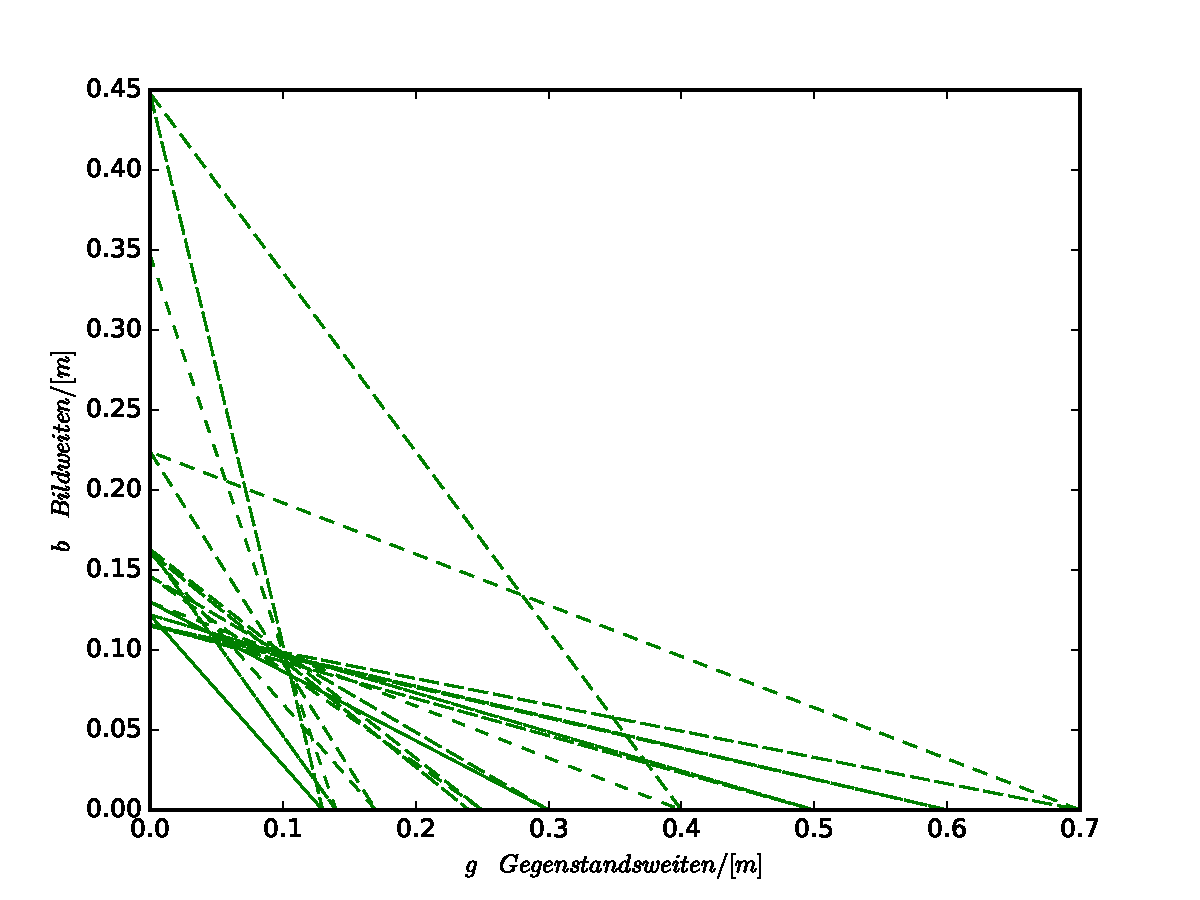
\includegraphics[height = 6cm]{plots/100mmLinsegbplot.pdf}
      \caption{Die Wertepaare \texorpdfstring{$\left(g_i , b_i \right)$}{math}
       für die Linse mit einer Brennweite von 100mm wurden in diesem
       Koordinatensystem eingetragen und durch eine Gerade verbunden. }
      \label{fig:Lgb}
    \end{subfigure}
    \begin{subfigure}{0.48\textwidth}
      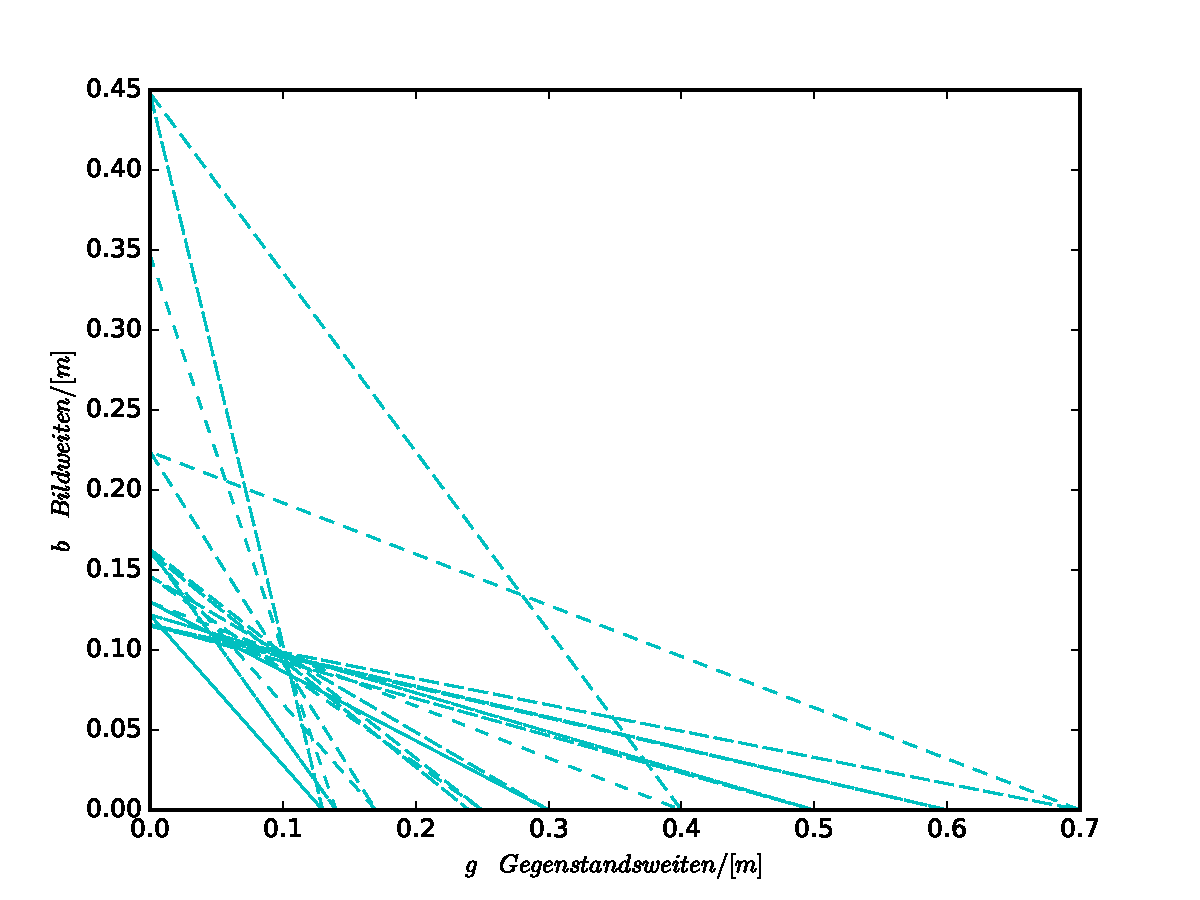
\includegraphics[height = 6cm]{plots/Wasserlinsegbplot.pdf}
      \caption{Die Wertepaare \texorpdfstring{$\left(g_i , b_i \right)$}{math}
       für die Wasserlinse wurden in diesem Koordinatensystem eingetragen und durch eine Gerade verbunden. }
      \label{fig:Wgb}
    \end{subfigure}
    \caption{Darstellungen zur Bestimmung der Brennweite über Gegenstands- und Bildweite.}
    \label{fig:gb}
\end{figure}
\FloatBarrier

\begin{table}
  \centering
  \sisetup{round-mode = places , round-precision = 2}
  \resizebox{\textwidth}{!}{
  \begin{tabular}{S S S S S S}
    \toprule
    $\text{xG}/\si{\meter}$ & $\text{xL}/\si{\meter} $ &
     $\text{xS} / \si{\meter}$ & $\text{g} / \si{\meter}$ &
     $\text{b}/\si{\meter} $ & $\text{f}_L / \si{\meter} $\\
    \midrule
    1.150000000000000133e+00 & 1.010000000000000009e+00 & 6.630000000000000338e-01 & 1.400000000000001243e-01 & 3.469999999999999751e-01 & 9.975359342915818273e-02\\
    1.150000000000000133e+00 & 9.000000000000000222e-01 & 7.369999999999999885e-01 & 2.500000000000001110e-01 & 1.630000000000000338e-01 & 9.866828087167073269e-02\\
    1.199999999999999956e+00 & 9.000000000000000222e-01 & 7.540000000000001146e-01 & 2.999999999999999334e-01 & 1.459999999999999076e-01 & 9.820627802690577723e-02\\
    1.199999999999999956e+00 & 8.000000000000000444e-01 & 6.700000000000000400e-01 & 3.999999999999999112e-01 & 1.300000000000000044e-01 & 9.811320754716981729e-02\\
    1.199999999999999956e+00 & 1.070000000000000062e+00 & 6.219999999999999973e-01 & 1.299999999999998934e-01 & 4.480000000000000648e-01 & 1.007612456747404295e-01\\
    1.199999999999999956e+00 & 7.000000000000000666e-01 & 5.779999999999999583e-01 & 4.999999999999998890e-01 & 1.220000000000001084e-01 & 9.807073954983930308e-02\\
    1.199999999999999956e+00 & 5.999999999999999778e-01 & 4.839999999999999858e-01 & 5.999999999999999778e-01 & 1.159999999999999920e-01 & 9.720670391061451976e-02\\
    1.199999999999999956e+00 & 5.000000000000000000e-01 & 3.850000000000000089e-01 & 6.999999999999999556e-01 & 1.149999999999999911e-01 & 9.877300613496931003e-02\\
    1.199999999999999956e+00 & 1.030000000000000027e+00 & 8.059999999999999387e-01 & 1.699999999999999289e-01 & 2.240000000000000879e-01 & 9.664974619289339042e-02\\
    1.277000000000000135e+00 & 1.037000000000000144e+00 & 8.760000000000000009e-01 & 2.399999999999999911e-01 & 1.610000000000001430e-01 & 9.635910224438908045e-02\\
    \bottomrule
  \end{tabular}
  }
  \caption{Werte zur Bestimmung der Gegenstadsweiten (g), der Bildweite (b)
  und der Brennweite (f), xG ist die Postion des Gegenstands, xL die Position der Linse
  und xS die Postion des Schirms, für die Linse mit Brennweite 100mm. }
  \label{tab:Lgb}
\end{table}
\begin{table}
  \centering
  \sisetup{round-mode = places , round-precision = 2}
  \resizebox{\textwidth}{!}{
  \begin{tabular}{S S S S S S}
    \toprule
    $\text{xG}/\si{\meter}$ & $\text{xL}/\si{\meter} $ &
     $\text{xS} / \si{\meter}$ & $\text{g} / \si{\meter}$ &
     $\text{b}/\si{\meter} $ & $\text{f}_W / \si{\meter} $\\
    \midrule
    1.250000000000000000e+00 & 1.167000000000000037e+00 & 9.609999999999999654e-01 & 8.299999999999996270e-02 & 2.060000000000000719e-01 & 5.916262975778545374e-02\\
    1.250000000000000000e+00 & 1.060000000000000053e+00 & 9.320000000000000506e-01 & 1.899999999999999467e-01 & 1.280000000000000027e-01 & 7.647798742138364747e-02\\
    1.250000000000000000e+00 & 1.010000000000000009e+00 & 8.940000000000001279e-01 & 2.399999999999999911e-01 & 1.159999999999998810e-01 & 7.820224719101116773e-02\\
    1.250000000000000000e+00 & 9.400000000000000577e-01 & 8.379999999999999671e-01 & 3.099999999999999423e-01 & 1.020000000000000906e-01 & 7.674757281553402921e-02\\
    1.250000000000000000e+00 & 9.599999999999999645e-01 & 8.540000000000000924e-01 & 2.900000000000000355e-01 & 1.059999999999998721e-01 & 7.762626262626255713e-02\\
    1.250000000000000000e+00 & 1.040000000000000036e+00 & 9.159999999999999254e-01 & 2.099999999999999645e-01 & 1.240000000000001101e-01 & 7.796407185628746739e-02\\
    1.250000000000000000e+00 & 1.100000000000000089e+00 & 9.400000000000000577e-01 & 1.499999999999999112e-01 & 1.600000000000000311e-01 & 7.741935483870965307e-02\\
    1.250000000000000000e+00 & 1.120000000000000107e+00 & 9.250000000000000444e-01 & 1.299999999999998934e-01 & 1.950000000000000622e-01 & 7.799999999999997213e-02\\
    1.250000000000000000e+00 & 1.140000000000000124e+00 & 8.780000000000000027e-01 & 1.099999999999998757e-01 & 2.620000000000001217e-01 & 7.747311827956984698e-02\\
    1.250000000000000000e+00 & 9.799999999999999822e-01 & 8.659999999999999920e-01 & 2.700000000000000178e-01 & 1.139999999999999902e-01 & 8.015624999999999833e-02\\
    \bottomrule
  \end{tabular}
  }
  \caption{Werte der zur Bestimmung der Gegenstadsweiten (g), der Bildweite (b)
  und der Brennweite (f), xG ist die Postion des Gegenstands, xL die Position der Linse
  und xS die Postion des Schirms für die Wasserlinse.}
  \label{tab:Wgb}
\end{table}
\begin{table}
  \centering
  \sisetup{round-mode = places , round-precision = 2}
  \resizebox{\textwidth}{!}{
  \begin{tabular}{S S S S S S}
    \toprule
    $\text{xG}/\si{\meter}$ & $\text{xL}/\si{\meter} $ &
     $\text{xS} / \si{\meter}$ & $\text{g} / \si{\meter}$ &
     $\text{b}/\si{\meter} $ & $\text{B} / \si{\meter} $\\
    \midrule
    1.150000000000000133e+00 & 1.010000000000000009e+00 & 6.630000000000000338e-01 & 1.400000000000001243e-01 & 3.469999999999999751e-01 & 7.200000000000000844e-02\\
    1.150000000000000133e+00 & 9.000000000000000222e-01 & 7.369999999999999885e-01 & 2.500000000000001110e-01 & 1.630000000000000338e-01 & 1.899999999999999953e-02\\
    1.199999999999999956e+00 & 9.000000000000000222e-01 & 7.540000000000001146e-01 & 2.999999999999999334e-01 & 1.459999999999999076e-01 & 1.399999999999999856e-02\\
    1.199999999999999956e+00 & 8.000000000000000444e-01 & 6.700000000000000400e-01 & 3.999999999999999112e-01 & 1.300000000000000044e-01 & 1.000000000000000021e-02\\
    1.199999999999999956e+00 & 1.070000000000000062e+00 & 6.219999999999999973e-01 & 1.299999999999998934e-01 & 4.480000000000000648e-01 & 1.000000000000000056e-01\\
    \bottomrule
  \end{tabular}
  }
  \caption{Werte der zur Bestimmung der Gegenstadsweiten (g) und der Bildweite (b),
  xG ist die Postion des Gegenstands, xL die Position der Linse,
  xS die Postion des Schirms und B ist die Bildgröße für die Linse mit Brennweite
  100mm.}
  \label{tab:Bgb}
\end{table}

\FloatBarrier
\subsection{Bestimmung der Brennweite nach der Methode von Bessel.}
Die Brennweiten werden nach der Fromel \eqref{eqn:bessel} bestimmt und
gemittelt. Dann ergibt sich für die mittlere Brennweite für weißes Licht
\begin{equation*}
  \bar{f_n} = \SI{0.04(06)}{\meter}
\end{equation*}
und  für die mittlere Brennweite für rotes $\bar{f_r}$ als auch blaues
$\bar{f_b}$ Licht
\begin{equation*}
  \bar{f_r} = \bar{f_b} = \SI{0.034(6)}{\meter} \; .
\end{equation*}
Alle Werte dazu sind in den Tabellen \ref{tab:bn} , \ref{tab:bb} und \ref{tab:br}
dargestellt. Fest zuhalten ist, dass die Brennweiten für rotes und blaues Licht
kleiner sind als die für normales Licht. Auch hier wurde wieder mit einer Linse
mit einer Brennweite von \SI{100}{\milli\meter} gearbeitet.
\begin{table}
  \centering
  \sisetup{round-mode = places , round-precision = 2}
  \resizebox{\textwidth}{!}{%
  \begin{tabular}{S S S S S S S}
    \toprule
    $\text{xG}/\si{\centi\meter}$ & $\text{xL}_{1} /\si{\centi\meter} $ &
    $\text{xL}_{2} /\si{\centi\meter} $ &
     $\text{xS} / \si{\centi\meter}$ & $\text{e}_n / \si{\meter}$ &
     $\text{d}_n /\si{\meter} $ & $\text{f}_n / \si{\meter} $\\
    \midrule
    1.250000000000000000e+02 & 7.229999999999999716e+01 & 1.122000000000000028e+02 & 6.000000000000000000e+01 & 6.500000000000000222e-01 & 3.990000000000000768e-01 & 4.278608749999999322e-02\\
    1.250000000000000000e+02 & 7.709999999999999432e+01 & 1.120000000000000000e+02 & 6.500000000000000000e+01 & 5.999999999999999778e-01 & 3.490000000000000879e-01 & 3.572984999999998662e-02\\
    1.250000000000000000e+02 & 8.309999999999999432e+01 & 1.115999999999999943e+02 & 7.000000000000000000e+01 & 5.500000000000000444e-01 & 2.850000000000000311e-01 & 3.042531250000000617e-02\\
    1.250000000000000000e+02 & 8.879999999999999716e+01 & 1.107999999999999972e+02 & 7.500000000000000000e+01 & 5.000000000000000000e-01 & 2.200000000000000011e-01 & 2.520000000000000018e-02\\
    1.250000000000000000e+02 & 9.440000000000000568e+01 & 1.102999999999999972e+02 & 8.000000000000000000e+01 & 4.500000000000000111e-01 & 1.589999999999999192e-01 & 1.993713750000000381e-02\\
    1.250000000000000000e+02 & 1.024000000000000057e+02 & 1.070999999999999943e+02 & 8.500000000000000000e+01 & 4.000000000000000222e-01 & 4.699999999999988909e-02 & 1.577910000000000423e-02\\
    1.250000000000000000e+02 & 5.150000000000000000e+01 & 1.140000000000000000e+02 & 4.000000000000000000e+01 & 8.499999999999999778e-01 & 6.250000000000000000e-01 & 7.052343749999998024e-02\\
    1.250000000000000000e+02 & 5.639999999999999858e+01 & 1.137999999999999972e+02 & 4.500000000000000000e+01 & 8.000000000000000444e-01 & 5.739999999999999547e-01 & 6.210480000000004330e-02\\
    1.250000000000000000e+02 & 6.160000000000000142e+01 & 1.137000000000000028e+02 & 5.000000000000000000e+01 & 7.500000000000000000e-01 & 5.210000000000000187e-01 & 5.457356249999999187e-02\\
    1.250000000000000000e+02 & 6.700000000000000000e+01 & 1.135000000000000000e+02 & 5.500000000000000000e+01 & 7.000000000000000666e-01 & 4.650000000000000244e-01 & 4.791062500000001917e-02\\
    \bottomrule
  \end{tabular}
  }
  \caption{Werte der zur Bestimmung der Brennweite \texorpdfstring{$f_n$}{math},
  xG ist die Postion des Gegenstands, \texorpdfstring{$\text{xL}_1$}{math}
  die erste Position der Linse, \texorpdfstring{$\text{xL}_2$}{math} die zweite
  Position der Linse und xS die Postion des Schirms für normales Licht.}
  \label{tab:bn}
\end{table}
\begin{table}
  \centering
  \sisetup{round-mode = places , round-precision = 2}
  \resizebox{\textwidth}{!}{
  \begin{tabular}{S S S S S S S}
    \toprule
    $\text{xG}/\si{\centi\meter}$ & $\text{xL}_{1} /\si{\centi\meter} $ &
    $\text{xL}_{2} /\si{\centi\meter} $ &
     $\text{xS} / \si{\centi\meter}$ & $\text{e}_b / \si{\meter}$ &
     $\text{d}_b /\si{\meter} $ & $\text{f}_b / \si{\meter} $\\
    \midrule
    1.250000000000000000e+02 & 1.125999999999999943e+02 & 6.700000000000000000e+01 & 5.500000000000000000e+01 & 7.000000000000000666e-01 & 4.559999999999999609e-01 & 4.936120000000002866e-02\\
    1.250000000000000000e+02 & 1.124000000000000057e+02 & 7.240000000000000568e+01 & 6.000000000000000000e+01 & 6.500000000000000222e-01 & 4.000000000000000222e-01 & 4.265625000000000666e-02\\
    1.250000000000000000e+02 & 1.122999999999999972e+02 & 7.750000000000000000e+01 & 6.500000000000000000e+01 & 5.999999999999999778e-01 & 3.479999999999999760e-01 & 3.583439999999999542e-02\\
    1.250000000000000000e+02 & 1.117000000000000028e+02 & 8.820000000000000284e+01 & 7.500000000000000000e+01 & 5.000000000000000000e-01 & 2.350000000000000144e-01 & 2.434687499999999699e-02\\
    1.250000000000000000e+02 & 1.085000000000000000e+02 & 1.020999999999999943e+02 & 8.500000000000000000e+01 & 4.000000000000000222e-01 & 6.400000000000005684e-02 & 1.559040000000000252e-02\\
    \bottomrule
  \end{tabular}
  }
  \caption{Werte der zur Bestimmung der Brennweite \texorpdfstring{$f_b$}{math},
  xG ist die Postion des Gegenstands, \texorpdfstring{$\text{xL}_1$}{math}
  die erste Position der Linse, \texorpdfstring{$\text{xL}_2$}{math} die zweite
  Position der Linse und xS die Postion des Schirms für blaues Licht.}
  \label{tab:bb}
\end{table}
\begin{table}
  \centering
  \sisetup{round-mode = places , round-precision = 2}
  \resizebox{\textwidth}{!}{
  \begin{tabular}{S S S S S S S}
    \toprule
    $\text{xG}/\si{\centi\meter}$ & $\text{xL}_{1} /\si{\centi\meter} $ &
    $\text{xL}_{2} /\si{\centi\meter} $ &
     $\text{xS} / \si{\centi\meter}$ & $\text{e}_r / \si{\meter}$ &
     $\text{d}_r /\si{\meter} $ & $\text{f}_r / \si{\meter} $\\
    \midrule
    1.250000000000000000e+02 & 1.020999999999999943e+02 & 1.077000000000000028e+02 & 8.500000000000000000e+01 & 4.000000000000000222e-01 & 5.600000000000008443e-02 & 1.568640000000000312e-02\\
    1.250000000000000000e+02 & 8.859999999999999432e+01 & 1.112000000000000028e+02 & 7.500000000000000000e+01 & 5.000000000000000000e-01 & 2.260000000000000897e-01 & 2.486549999999999525e-02\\
    1.250000000000000000e+02 & 7.750000000000000000e+01 & 1.120999999999999943e+02 & 6.500000000000000000e+01 & 5.999999999999999778e-01 & 3.459999999999999742e-01 & 3.604260000000000103e-02\\
    1.250000000000000000e+02 & 7.240000000000000568e+01 & 1.125000000000000000e+02 & 6.000000000000000000e+01 & 6.500000000000000222e-01 & 4.009999999999999676e-01 & 4.252608750000001075e-02\\
    1.250000000000000000e+02 & 6.709999999999999432e+01 & 1.125999999999999943e+02 & 5.500000000000000000e+01 & 7.000000000000000666e-01 & 4.550000000000000155e-01 & 4.952062500000001949e-02\\
    \bottomrule
  \end{tabular}
  }
  \caption{Werte der zur Bestimmung der Brennweite \texorpdfstring{$f_r$}{math},
  xG ist die Postion des Gegenstands, \texorpdfstring{$\text{xL}_1$}{math}
  die erste Position der Linse, \texorpdfstring{$\text{xL}_2$}{math} die zweite
  Position der Linse und xS die Postion des Schirms für rotes Licht.}
  \label{tab:br}
\end{table}




\FloatBarrier
\subsection{Bestimmung der Brennweite eines Linsensystems nach der Methode von Abbe.}

\begin{figure}
  \centering
    \begin{subfigure}{0.48\textwidth}
      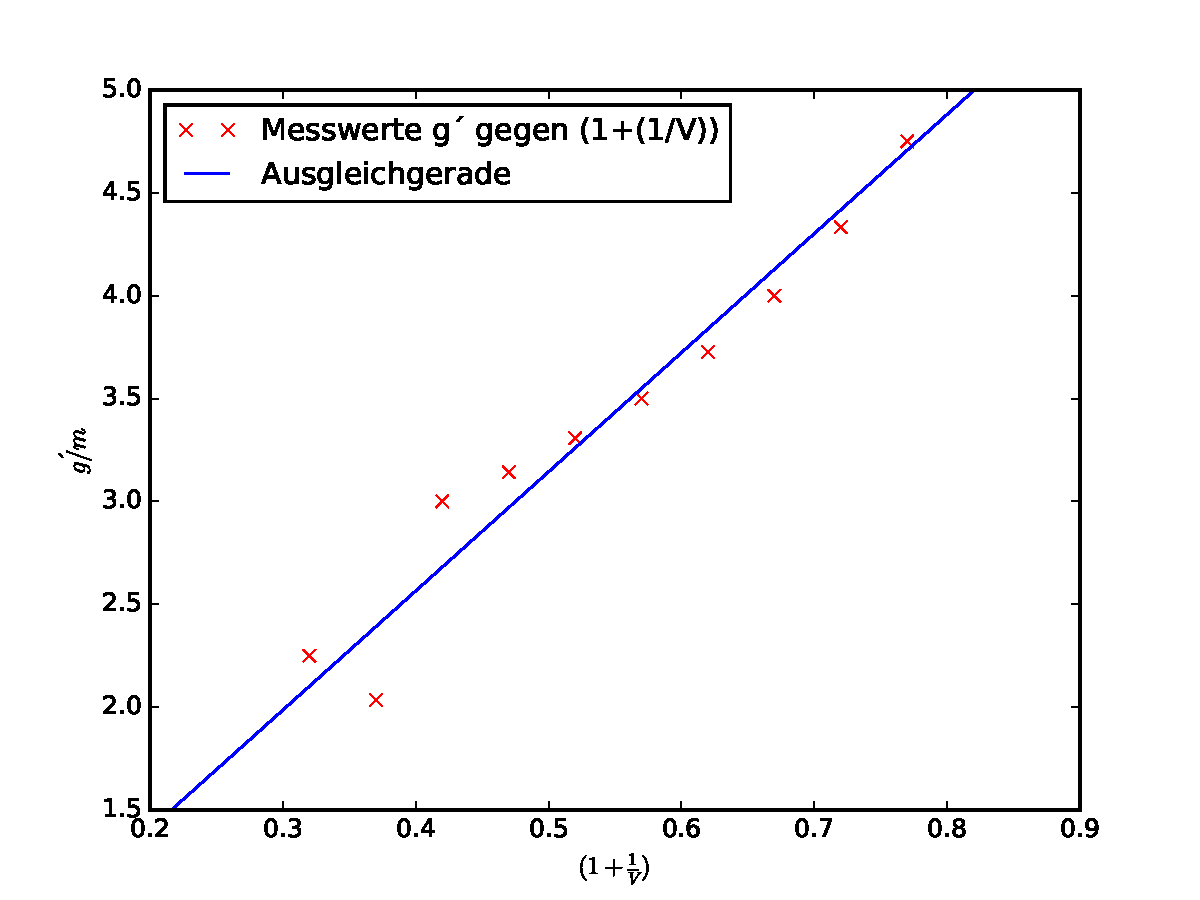
\includegraphics[height = 6cm]{plots/gsplot.pdf}
      \caption{In diesem Diagramm ist g' gegen
      \texorpdfstring{$\left(1 + \frac{1}{V}\right)$}{math} aufgetragen und
      eine Ausgleichgerade eingezeichnet. }
      \label{fig:Lgb}
    \end{subfigure}
    \begin{subfigure}{0.48\textwidth}
      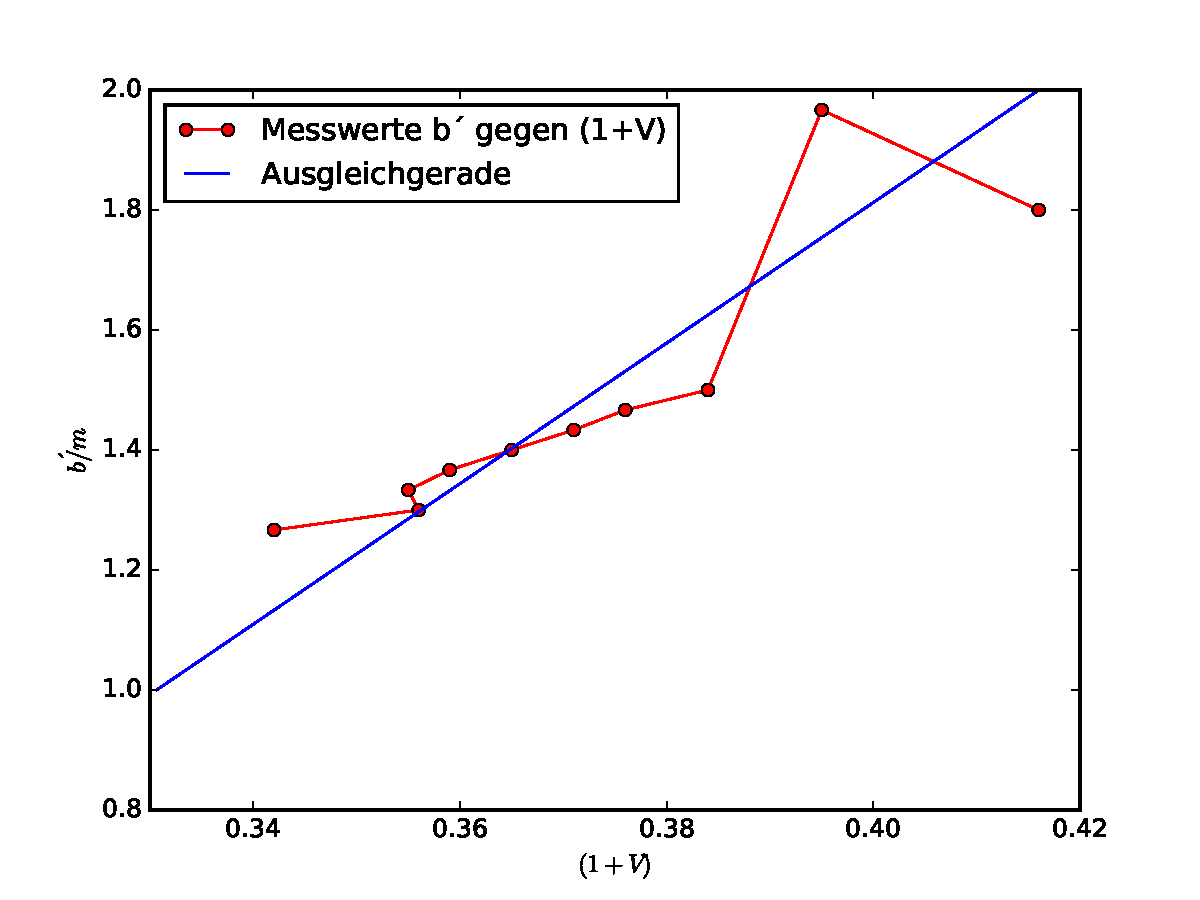
\includegraphics[height = 6cm]{plots/bsplot.pdf}
      \caption{In diesem Diagramm ist b' gegen (1 + V) aufgetragen und
      eine Ausgleichsgerade eingezeichnet. }
      \label{fig:Wgb}
    \end{subfigure}
    \caption{Diagramme zur Bestimmung der Brennweite eines Linsensystems nach Abbe.}
\end{figure}
